% --------------------------------------------------------------
% This is all preamble stuff that you don't have to worry about.
% Head down to where it says "Start here"
% --------------------------------------------------------------
 
\documentclass[12pt]{article}
 
\usepackage[margin=1in]{geometry} 
\usepackage{amsmath,amsthm,amssymb}
 
\newcommand{\N}{\mathbb{N}}
\newcommand{\Z}{\mathbb{Z}}
 
\newenvironment{theorem}[2][Theorem]{\begin{trivlist}
\item[\hskip \labelsep {\bfseries #1}\hskip \labelsep {\bfseries #2.}]}{\end{trivlist}}

\newenvironment{lemma}[2][Lemma]{\begin{trivlist}
\item[\hskip \labelsep {\bfseries #1}\hskip \labelsep {\bfseries #2.}]}{\end{trivlist}}

\newenvironment{exercise}[2][Exercise]{\begin{trivlist}
\item[\hskip \labelsep {\bfseries #1}\hskip \labelsep {\bfseries #2.}]}{\end{trivlist}}

\newenvironment{problem}[2][Problem]{\begin{trivlist}
\item[\hskip \labelsep {\bfseries #1}\hskip \labelsep {\bfseries #2}]}{\end{trivlist}}

\newenvironment{question}[2][Question]{\begin{trivlist}
\item[\hskip \labelsep {\bfseries #1}\hskip \labelsep {\bfseries #2.}]}{\end{trivlist}}

\newenvironment{corollary}[2][Corollary]{\begin{trivlist}
\item[\hskip \labelsep {\bfseries #1}\hskip \labelsep {\bfseries #2.}]}{\end{trivlist}}

\usepackage{graphicx}
\graphicspath{{./}}

\begin{document}
 
% --------------------------------------------------------------
%                         Start here
% --------------------------------------------------------------
 
\title{Homework 3}%replace X with the appropriate number
\author{Yunzhong He\\ %replace with your name
204010749} %if necessary, replace with your course title
 
\maketitle
 
\begin{problem}{1}
\item{Q1}
Considering all training data (spam and ham), the most frequent 3 words are
\{(enron: 600), (will: 351), (please: 291)\}
\end{problem}

\begin{problem}{2}
\item{Q2}
For unregularized cross-entropy, we have
\begin{align*}
		w^{t+1} &= w^t - \alpha\frac{\partial\epsilon(w^t,b)}{\partial w^t_j} \\
		&= w^t +\alpha\sum_i (y_i \frac{1}{\sigma(b+w^{tT}x)}
		-(1-y_i)\frac{1}{1-\sigma(b+w^{tT}x)}) \frac{\partial\sigma(b+w^{tT}x)}{\partial w^t_j}) \\
		&= w^t +\alpha\sum_i(y_i-\sigma(b+w^{tT}x))x_j \\
		b^{t+1} &= b^t + \alpha\sum_i(y_i-\sigma(b+w^{tT}x))
\end{align*}
Similarly, for adding regularization term, we have
\begin{align*}
		w^{t+1} &= w^t - \alpha\frac{\partial\epsilon_{regularized}(w^t,b)}{\partial w^t_j}\\
		&= w +\alpha(\sum_i(y_i-\sigma(b+w^Tx))x_j) + 2 \lambda w_j)\\
		b^{t+1} &= b^t + \alpha\sum_i(y_i-\sigma(b+w^{tT}x))
\end{align*}
For the implementation $b$ is merged into $w$ by adding a constant 1 into $x$.
\end{problem}

\begin{problem}{3.1 Batch Gradient Descent}
\item{Q3 a.}
Running gradient descent without regularization on the ionosphere dataset with 50 iterations, we have the following result for ionosphere classification.
\begin{center}
		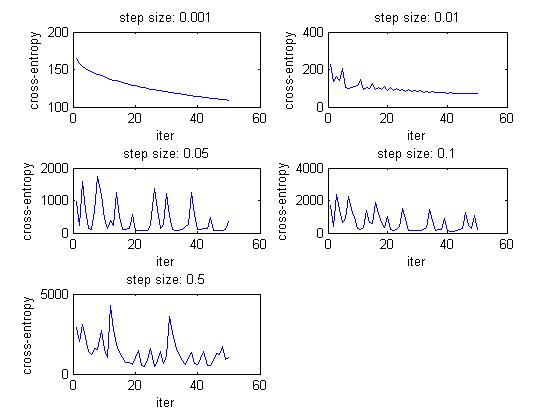
\includegraphics[height=12.5cm]{ionosphere_gradient_descent.jpg}{\\fig.1 ionosphere no regularizatoin}
\end{center}
And we obtained the following results for spam classification.
\begin{center}
		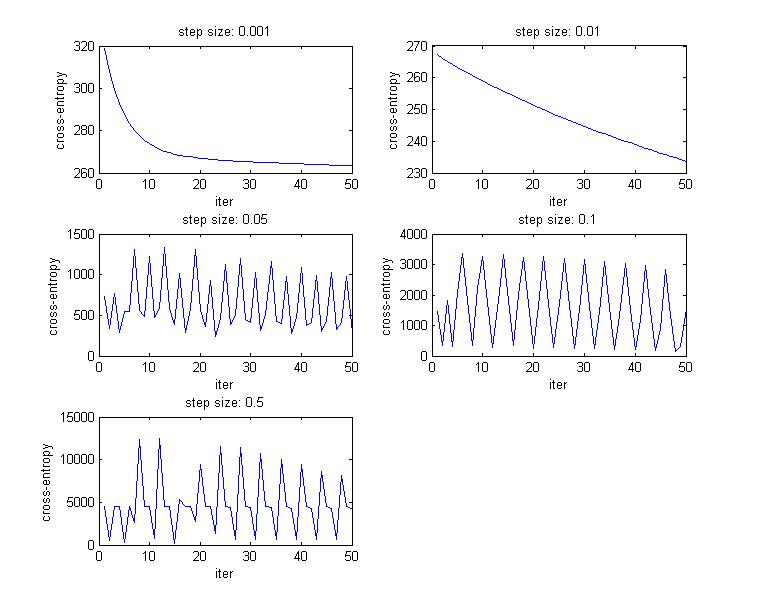
\includegraphics[height=12.5cm]{spams_gradient_descent.jpg}{\\fig.2 spam no regularizatoin}
\end{center}
\clearpage
\item{Q3 b.}
The L2 norms without regulazation are below
\begin{center}
	\begin{tabular}{||c c c c c c||} 
		\hline
	   	L2 norm (no regularization) & 0.001 & 0.01 & 0.05 & 0.1 & 0.5 \\ [0.5ex] 
		\hline
		ionosphere & 1.5401 & 5.4345 & 21.563 & 43.828 & 216.15 \\
		\hline
		spam & 1.1171 & 4.2402 & 19.359 & 41.603 & 210.54 \\
		\hline
	\end{tabular}
\end{center}
\item{Q4 a.}
Running gradient descent with regularization on the ionosphere dataset with 50 iterations, we have the following result.
\begin{center}
		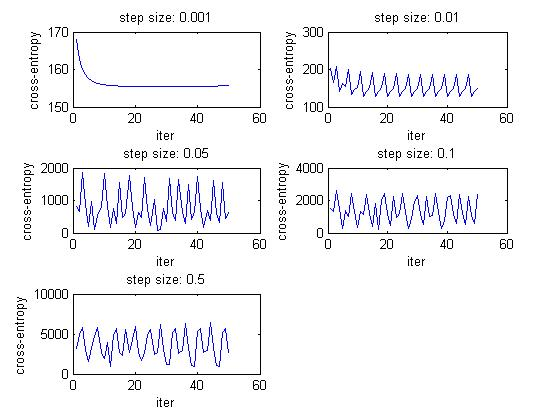
\includegraphics[height=12.5cm]{ionosphere_gradient_descent_regularized.jpg}{\\fig.3 ionosphere with regularization}
\end{center}
And we obtained the following results for spam classification.
\begin{center}
		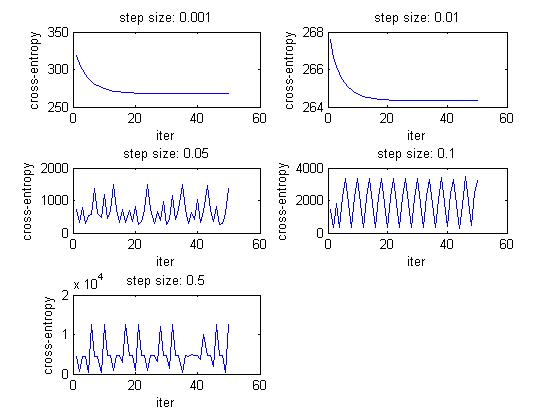
\includegraphics[height=12.5cm]{spams_gradient_descent_regularized.jpg}{\\fig.4 spam with regularization}
\end{center}
\item{Q4 b.}
The L2 norms with regulazation are below
\begin{center}
	\begin{tabular}{||c c c c c c||} 
		\hline
	   	L2 norm (with regularization) & 0.001 & 0.01 & 0.05 & 0.1 & 0.5 \\ [0.5ex] 
		\hline
		ionosphere & 0.32193 & 1.6173 & 7.2724 & 33.345 & 86.251 \\
		\hline
		spam & 1.0094 & 1.0849 & 11.484 & 26.894 & 43.607 \\
		\hline
	\end{tabular}
\end{center}
\item{Q4 c.}
Plotting the final cross-entropy with training and test data set together with different parameters, we have the following graphs. Notice that the training cross-entropy for ionosphere is larger than teting's, because there are more points in the training set. If we normalize the values with their numbers, it will be smaller.
\begin{center}
		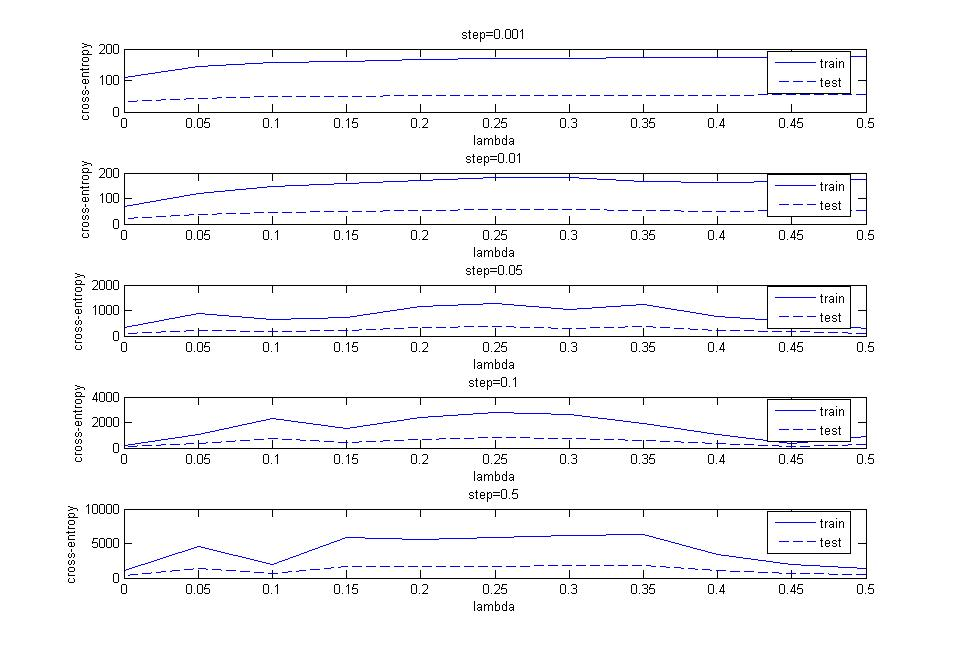
\includegraphics[height=12.5cm]{ionosphere_4c.jpg}{\\fig.5 cross-entropy with different parameters - ionosphere}
\end{center}
\begin{center}
		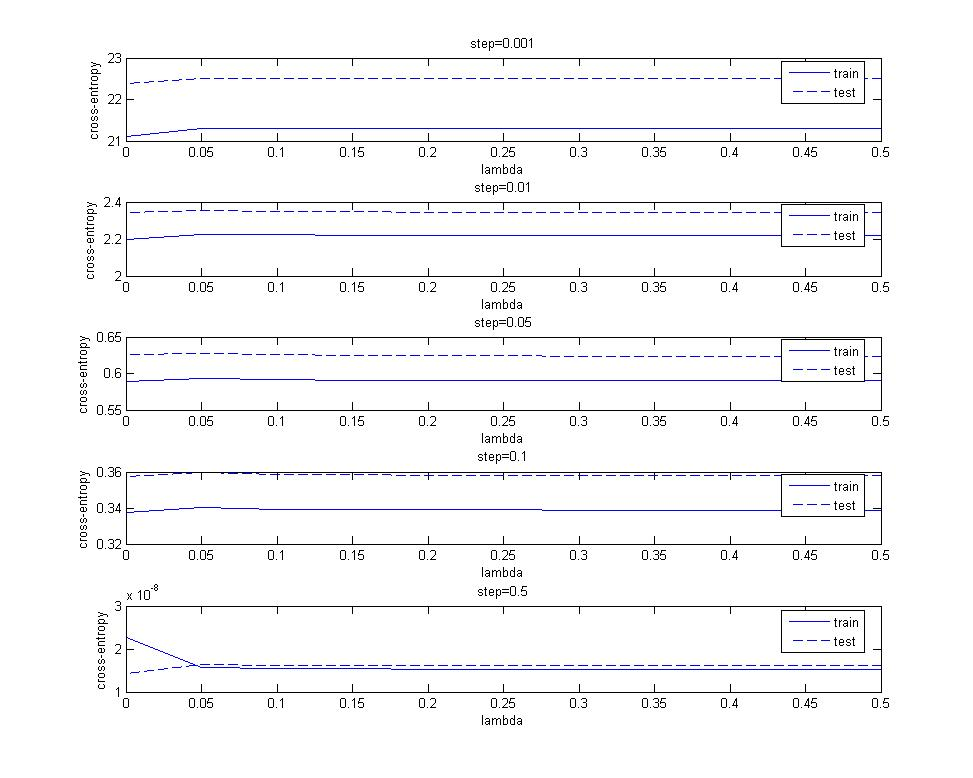
\includegraphics[height=12.5cm]{spams_4c.jpg}{\\fig.6 cross-entropy with different parameters - spam}
\end{center}
\end{problem}
\begin{problem} {3.2 Newton's Method}
\item{Q5}
Using Newton's method, assuming the $w$ is has length m, we have
	\begin{align*}
			&w^{t+1} = w^t - H^{-1}\epsilon(w, b) \nabla \epsilon(w, b) \\
			&b^{t+1} = b^t - (H^{-1}\epsilon(w, b) \nabla \epsilon(w, b))_{m+1}
	\end{align*}
where
	\begin{align*}
		&\nabla \epsilon(w, b)_j = \sum_i (\sigma(b+w^Tx) - y_i) \cdot x_j \\
		&H(\epsilon(w, b))_{jk} = \sum_i \sigma(b+w^Tx)(1-\sigma(b+w^Tx)) \cdot x_jx_k
	\end{align*}
similarly, adding regularization term we have
	\begin{align*}
			&w^{t+1} = w^t - H^{-1}\epsilon_{regularize}(w, b) \nabla \epsilon_{regulariz}(w, b) \\
			&b^{t+1} = b^t - (H^{-1}\epsilon(w, b) \nabla \epsilon(w, b))_{m+1}
	\end{align*}
where
	\begin{align*}
		&\nabla \epsilon_{regularize}(w, b)_j = \sum_i (\sigma(b+w^Tx) - y_i) \cdot x_j + 2 \lambda w_j \\
		&H(\epsilon_{regularize}(w, b))_{jk} = \sum_i \sigma(b+w^Tx)(1-\sigma(b+w^Tx)) \cdot x_jx_k \ \ \ (j \neq k)\\
		&H(\epsilon_{regularize}(w, b))_{jk} = \sum_i \sigma(b+w^Tx)(1-\sigma(b+w^Tx)) \cdot x_jx_k + 2 \lambda \ \ \ (j = k)
	\end{align*}
\item{Q6 a.}
Using Newton's method without regularization in ionosphere classification we have the following result.
\begin{center}
		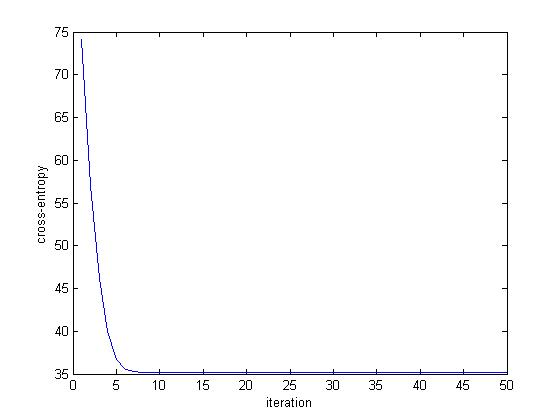
\includegraphics[height=8cm]{ionosphere_newtons.jpg}{\\fig.7 iosphere Newton's method no regularizatoin}
\end{center}
And with spam classification we have
\begin{center}
		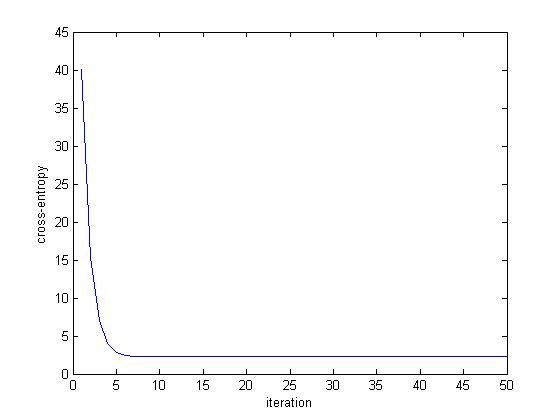
\includegraphics[height=8cm]{spams_newtons.jpg}{\\fig.8 spams Newton's method no regularization}
\end{center}.
\item{Q6 b}
	The L2 norm for ionosphere classification using Newton's method without regularization is \textbf{64.778}, and for spam classification we have \textbf{5665}.
\item{Q6 c}
	With the trained parameter w, we found the cross-entropy on test data to be \textbf{79.82} for ionosphere classification, and \textbf{2708}.
\item{Q7}
Adding different regularization parameters, we have the following results for ionosphere classification.
\begin{center}
	\begin{tabular}{||c c c||} 
		\hline
	   	$\lambda$ & L2 Norm  & regularized cross-entropy(test) \\
		\hline
	    0.00000 & 94.08943 & 79.81977\\
		\hline
	    0.05000 & 16.00648 & 40.07687\\
		\hline
	    0.10000 & 12.22773 & 36.30047\\
		\hline
	    0.15000 & 10.45439 & 35.11737\\
		\hline
	    0.20000 & 9.36224  & 34.81506\\
		\hline
	    0.25000 & 8.60089  & 34.89680\\
		\hline
	    0.30000 & 8.02942  & 35.15565\\
		\hline
	    0.35000 & 7.57861  & 35.49507\\
		\hline
	    0.40000 & 7.21010  & 35.86805\\
		\hline
	    0.45000 & 6.90076  & 36.25102\\
		\hline
	    0.50000 & 6.63567  & 36.63191\\
		\hline
	\end{tabular}
	{\\fig.9 Newton's method for ionosphere classification}
\end{center}
And for spam classification we have

\begin{center}
	\begin{tabular}{||c c c||} 
		\hline
	   	$\lambda$ & L2 Norm  & regularized cross-entropy(test) \\
		\hline
		0    &  3403.6 & 2708.56\\
		\hline
		0.05 &   26.83 & 224.559\\
		\hline
		0.1  &  18.187 & 238.623\\
		\hline
		0.15 &  14.221 & 246.204\\
		\hline
		0.2  & 11.8424 & 251.176\\
		\hline
		0.25 & 10.2263 & 254.760\\
		\hline
		0.3  & 9.0442  & 257.496\\
		\hline
		0.35 & 8.1361  & 259.667\\
		\hline
		0.4  & 7.4134  & 261.438\\
		\hline
		0.45 & 6.8226  & 262.915\\
		\hline
		0.5  & 6.3295  & 264.167\\
		\hline
	\end{tabular}
	{\\fig.10 Newton's method for spam classification}
\end{center}
Below the plots below show the progress of Newton's method with different $\lambda$ on the two data sets.
\begin{center}
		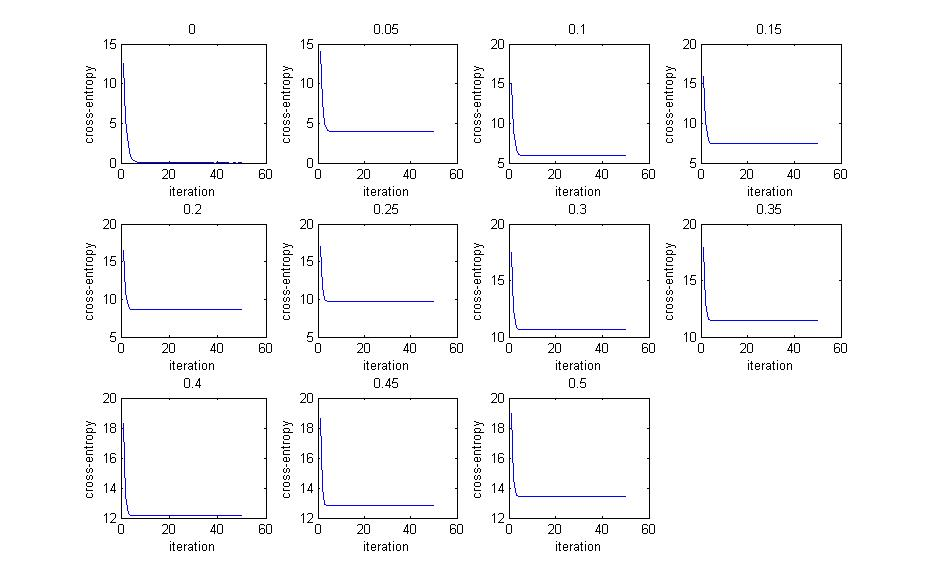
\includegraphics[height=12.5cm]{newtons_ionosphere.jpg}{\\fig.11 Newton's method with different $\lambda$ for ionosphere}
\end{center}
And we obtained the following results for spam classification.
\begin{center}
		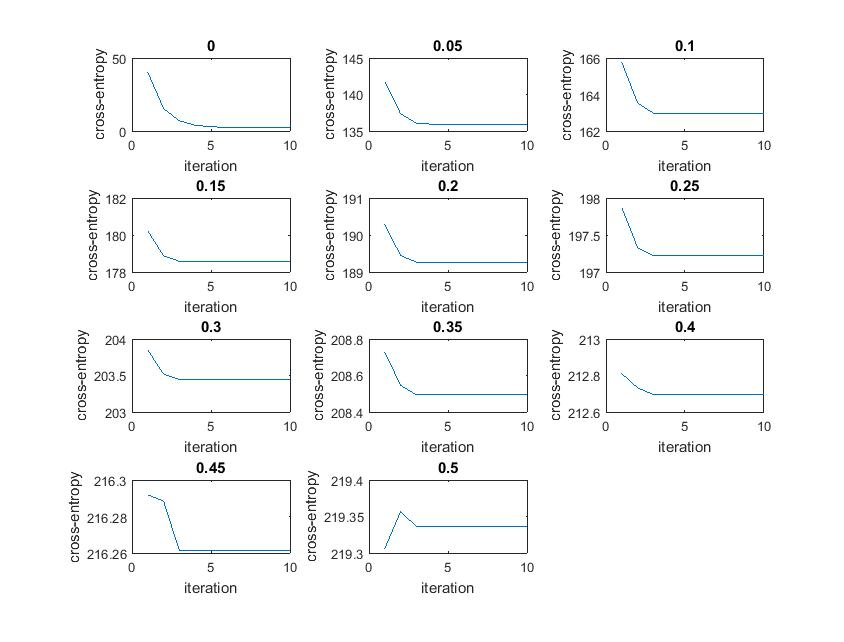
\includegraphics[height=12.5cm]{spam_newtons.jpg}{\\fig.12 Newton's method with different $\lambda$ for spams}
\end{center}
And we obtained the following results for spam classification.
\item{Q8}
From resutls in Q3 and Q4 we can see that gradient descent works pretty good when step size is 0.001 and 0.01, but starts to be zigzaging when step size is greater than 0.05, meaning $w$ starts to move back and forth around the optimal value. Also, when adding regularization, the testing cross-entropy becomes smaller along with L2 norm, indicating that without regularization we overfit the data.\\
\item{Q9}
Comparing Q4 and Q7 we can see that cross-entropy decreased significantly for training data, meaning that Newton's method does better in 50 iterations in finding the optimal. And this agrees with fig.7 and fig.8 where Newton's method converges much faster than gradient descent. But notice that in the spam case(fig.8/fig.10), for Newton's method without regularization, the training cross-entropy dropped to almost 0 while the testing cross-entropy becomes the largest among all other results. This suggests that there's a severe overfitting going on, and is fixed by adding regularizations into Newton's method.

\end{problem}


% --------------------------------------------------------------
%     You don't have to mess with anything below this line.
% --------------------------------------------------------------

\end{document}
